\begin{frame}
\frametitle{Company at a glance}
  \begin{columns}
  \column{0.73\textwidth}
  \small
  \begin{itemize}
    \item Engineering company created in 2004,\\
	  named "Free Electrons" until Feb. 2018.
    \item Locations: Orange, Toulouse, Lyon (France)
    \item Serving customers all around the world
    \item Head count: 13 - Only Free Software enthusiasts!
    \item Focus: Embedded Linux, Linux kernel,
          build systems and low level Free and Open Source Software
          for embedded and real-time systems.
    \item Feb. 2021: Bootlin is the 20th all-time Linux kernel contributor
    \item Activities: development, training, consulting, technical
          support.
    \item Added value: get the best of the user and development
          community and the resources it offers.
  \end{itemize}
  \column{0.27\textwidth}
  \includegraphics[width=\textwidth]{common/bootlin-logo.pdf}\\
  \vspace{0.25cm}
  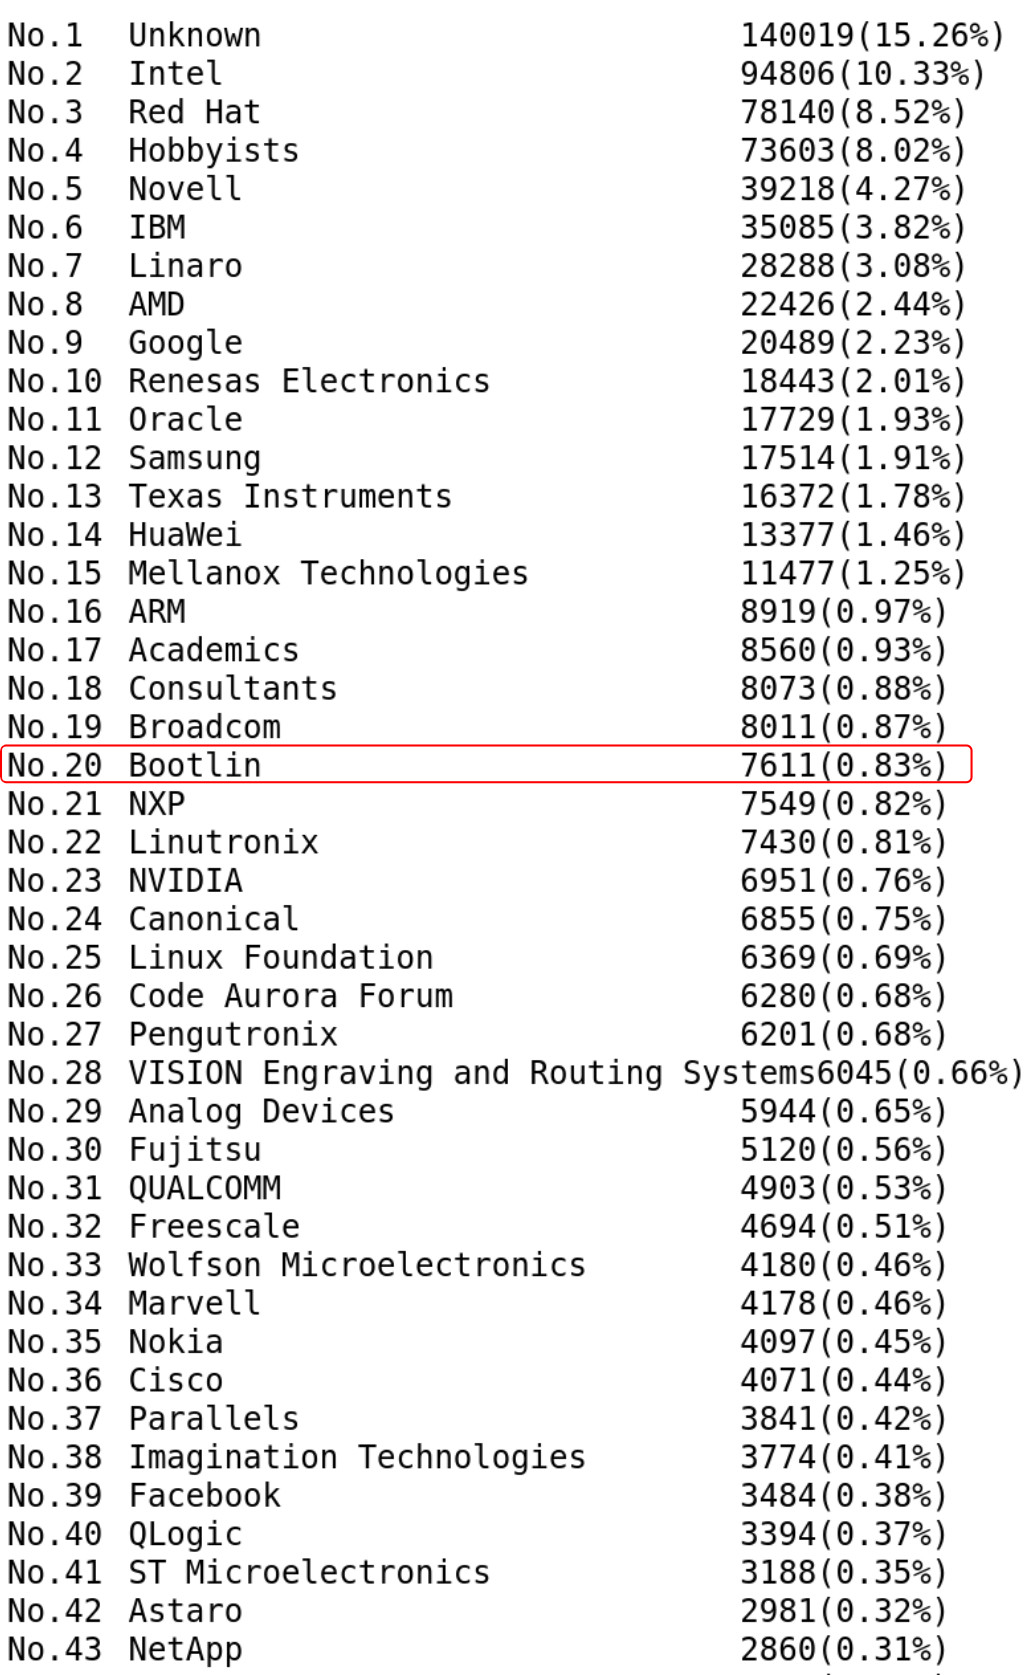
\includegraphics[width=0.95\textwidth]{slides/about-us/bootlin-kernel-contribs.jpg}\\
  \tiny Top Linux contributors since \code{git} (2005)
  \end{columns}
\end{frame}

\begin{frame}
\frametitle{Bootlin on-line resources}
\begin{columns}
\column{0.6\textwidth}
  \begin{itemize}
    \item All our training materials and technical presentations:\\
          \url{https://bootlin.com/docs/}
    \item Technical blog:\\
          \url{https://bootlin.com/}
    \item Quick news (Mastodon):\\
          \url{https://fosstodon.org/@bootlin}
    \item Quick news (Twitter):\\
          \url{https://twitter.com/bootlincom}
    \item Quick news (LinkedIn):\\
	  \url{https://www.linkedin.com/company/bootlin}
    \item Elixir - browse Linux kernel sources on-line:\\
          \url{https://elixir.bootlin.com}
  \end{itemize}
\column{0.4\textwidth}
  \includegraphics[width=\textwidth]{slides/about-us/mastodon.pdf}\\
  \vspace{3cm}
  \small Mastodon is a free and decentralized social network created
  in the best interests of its users.\\
  \vspace{0.5cm}
  \tiny Image credits: Jin Nguyen - \url{https://frama.link/bQwcWHTP}
\end{columns}
\end{frame}
